\documentclass[a4paper,12pt]{report}

%Package
\usepackage[utf8]{inputenc}         % acentos
\usepackage[francais]{babel}

 \usepackage{graphicx}
 \usepackage{caption}
 \usepackage{subcaption}
 \usepackage{fancyvrb}
 \usepackage{float}
 \usepackage{lscape}
 \usepackage{amsmath, bm}
 \usepackage{mathtools}
 \usepackage{epstopdf}
 \usepackage{multirow}
 \usepackage{amssymb}		
\usepackage[]{mcode}
\usepackage{tikz}

\DeclarePairedDelimiter{\ceil}{\lceil}{\rceil}
\DeclareUnicodeCharacter{00A0}{ }
\def\checkmark{\tikz\fill[scale=0.4](0,.35) -- (.25,0) -- (1,.7) -- (.25,.15) -- cycle;}
\graphicspath{{./figs/}}
\newcommand{\mat}[1]{\mbox{\boldmath{$#1$}}} 

\begin{document}
\begin{center}
	\large{ANALYSE D'IMAGES RADIOGRAPHIQUES DES POUMONS POUR L'AIDE AU DIAGNOSTIC}\\
	\vspace{2cm}
	\large{Camille Ruppli \\Renata Porciuncula Baptista}\\
\end{center}
\vspace{3cm}
\hspace{7cm}
\hfill \parbox{8.0cm}{Rapport du projet d'IMA 201\\Télécom Paristech\\}
\vspace{2cm}
\hfill \parbox{8.0cm}{Professeur Encadrement: Isabelle Bloch} \\
\vspace{2cm}
\begin{center}
	Paris
	
	Novembre de 2017
\end{center}

\tableofcontents
\begin{abstract}
	Le but de ce rapport est décrit les activités réalises par les étudiantes lorsque le développement d'une système dont l'objective est analyser d'images de radiographies pour identifier le tuberculose. La langage utilisée était \textit{Python2.7}.   
\end{abstract}

\chapter {Introduction}
Le but de ce projet est de reconnaître si un patient a tuberculose ou non, à partir de ses radiographies, en faisant une système automatique d'aide au diagnostic. Cette approche peut être utile, dans les régions où l'aces à des médecins est limité, en faisant une dépistage. Dans ce travail, les patients sont des enfants. La quantité totale des images disponibles était 8.

Le travail était divisé en trois parties qui seront décrit ci-dessous. Avant analyser quelque éléments dans le radiographies (RX), il a besoin de faire un pré traitement de les images pour isoler mieux les poumons, cela était le premier étape du travail.

Puis, quand il reste que les poumons, il est possible de commencer a analyser les images et apercevoir des éléments qui caractérisent une maladie. Ici, le objective était trouver irrégularités dans les poumons sans essayer de classifier cela comme tuberculose ou autre maladie.

Le troisième étape était trouver des caractéristiques qui sont spécifiques de le tuberculose. 

Le travail était implémenter en \textit{python} 2.7 en utilisant le bibliothèque \textit{opencv}.
\chapter {Développement}
\section{Détecter les poumons}
Le premier idée était utiliser qu'un méthode de détection des contours. La bibliothèque choisit a une fonction pour le faire, qui utilise le topologique algorithme. Une difficulté a été aperçu: cette approche donne comme résultat beaucoup de petits contours qui ne représente pas les vrais objets des images. Pour résoudre cela, une contrainte de taille a été appliquée. C'est possible d'observer les résultats initiales dans la Figure 2.1. 
 
\begin{figure}[ht]
	\begin{minipage}[b]{.5\textwidth}
		\centering
		\includegraphics[width=1\textwidth]{contours_Rx1anNormale.png}
		\subcaption{RX normale}
	\end{minipage}
	\hfill
	\begin{minipage}[b]{.46\textwidth}
		\centering
		\includegraphics[width=1\textwidth]{contours_Rx4_5ansPneumopathieNecrosanteDroite}
		\subcaption{RX tuberculose}
	\end{minipage}
\caption{Résultats: fonction \textit{findcontours} }
\end{figure}

Avec ces deux exemples, c'est possible noter la difficulté qui a suivi. Il n'est pas possible seulement utiliser ce détection de contours, parce que quand un poumon est beaucoup dégrade avec une maladie, le fonction dit que ce objet n'est plus un poumon. L'idée proposée, donc, c'était calculer le boîte englobant de le plus grand contour et tout qui était dehors ce boîte été mises en noie. Les résultat sont présentés dans la Figure 2.2.


\begin{figure}[ht]
	\begin{minipage}[b]{.5\textwidth}
		\centering
		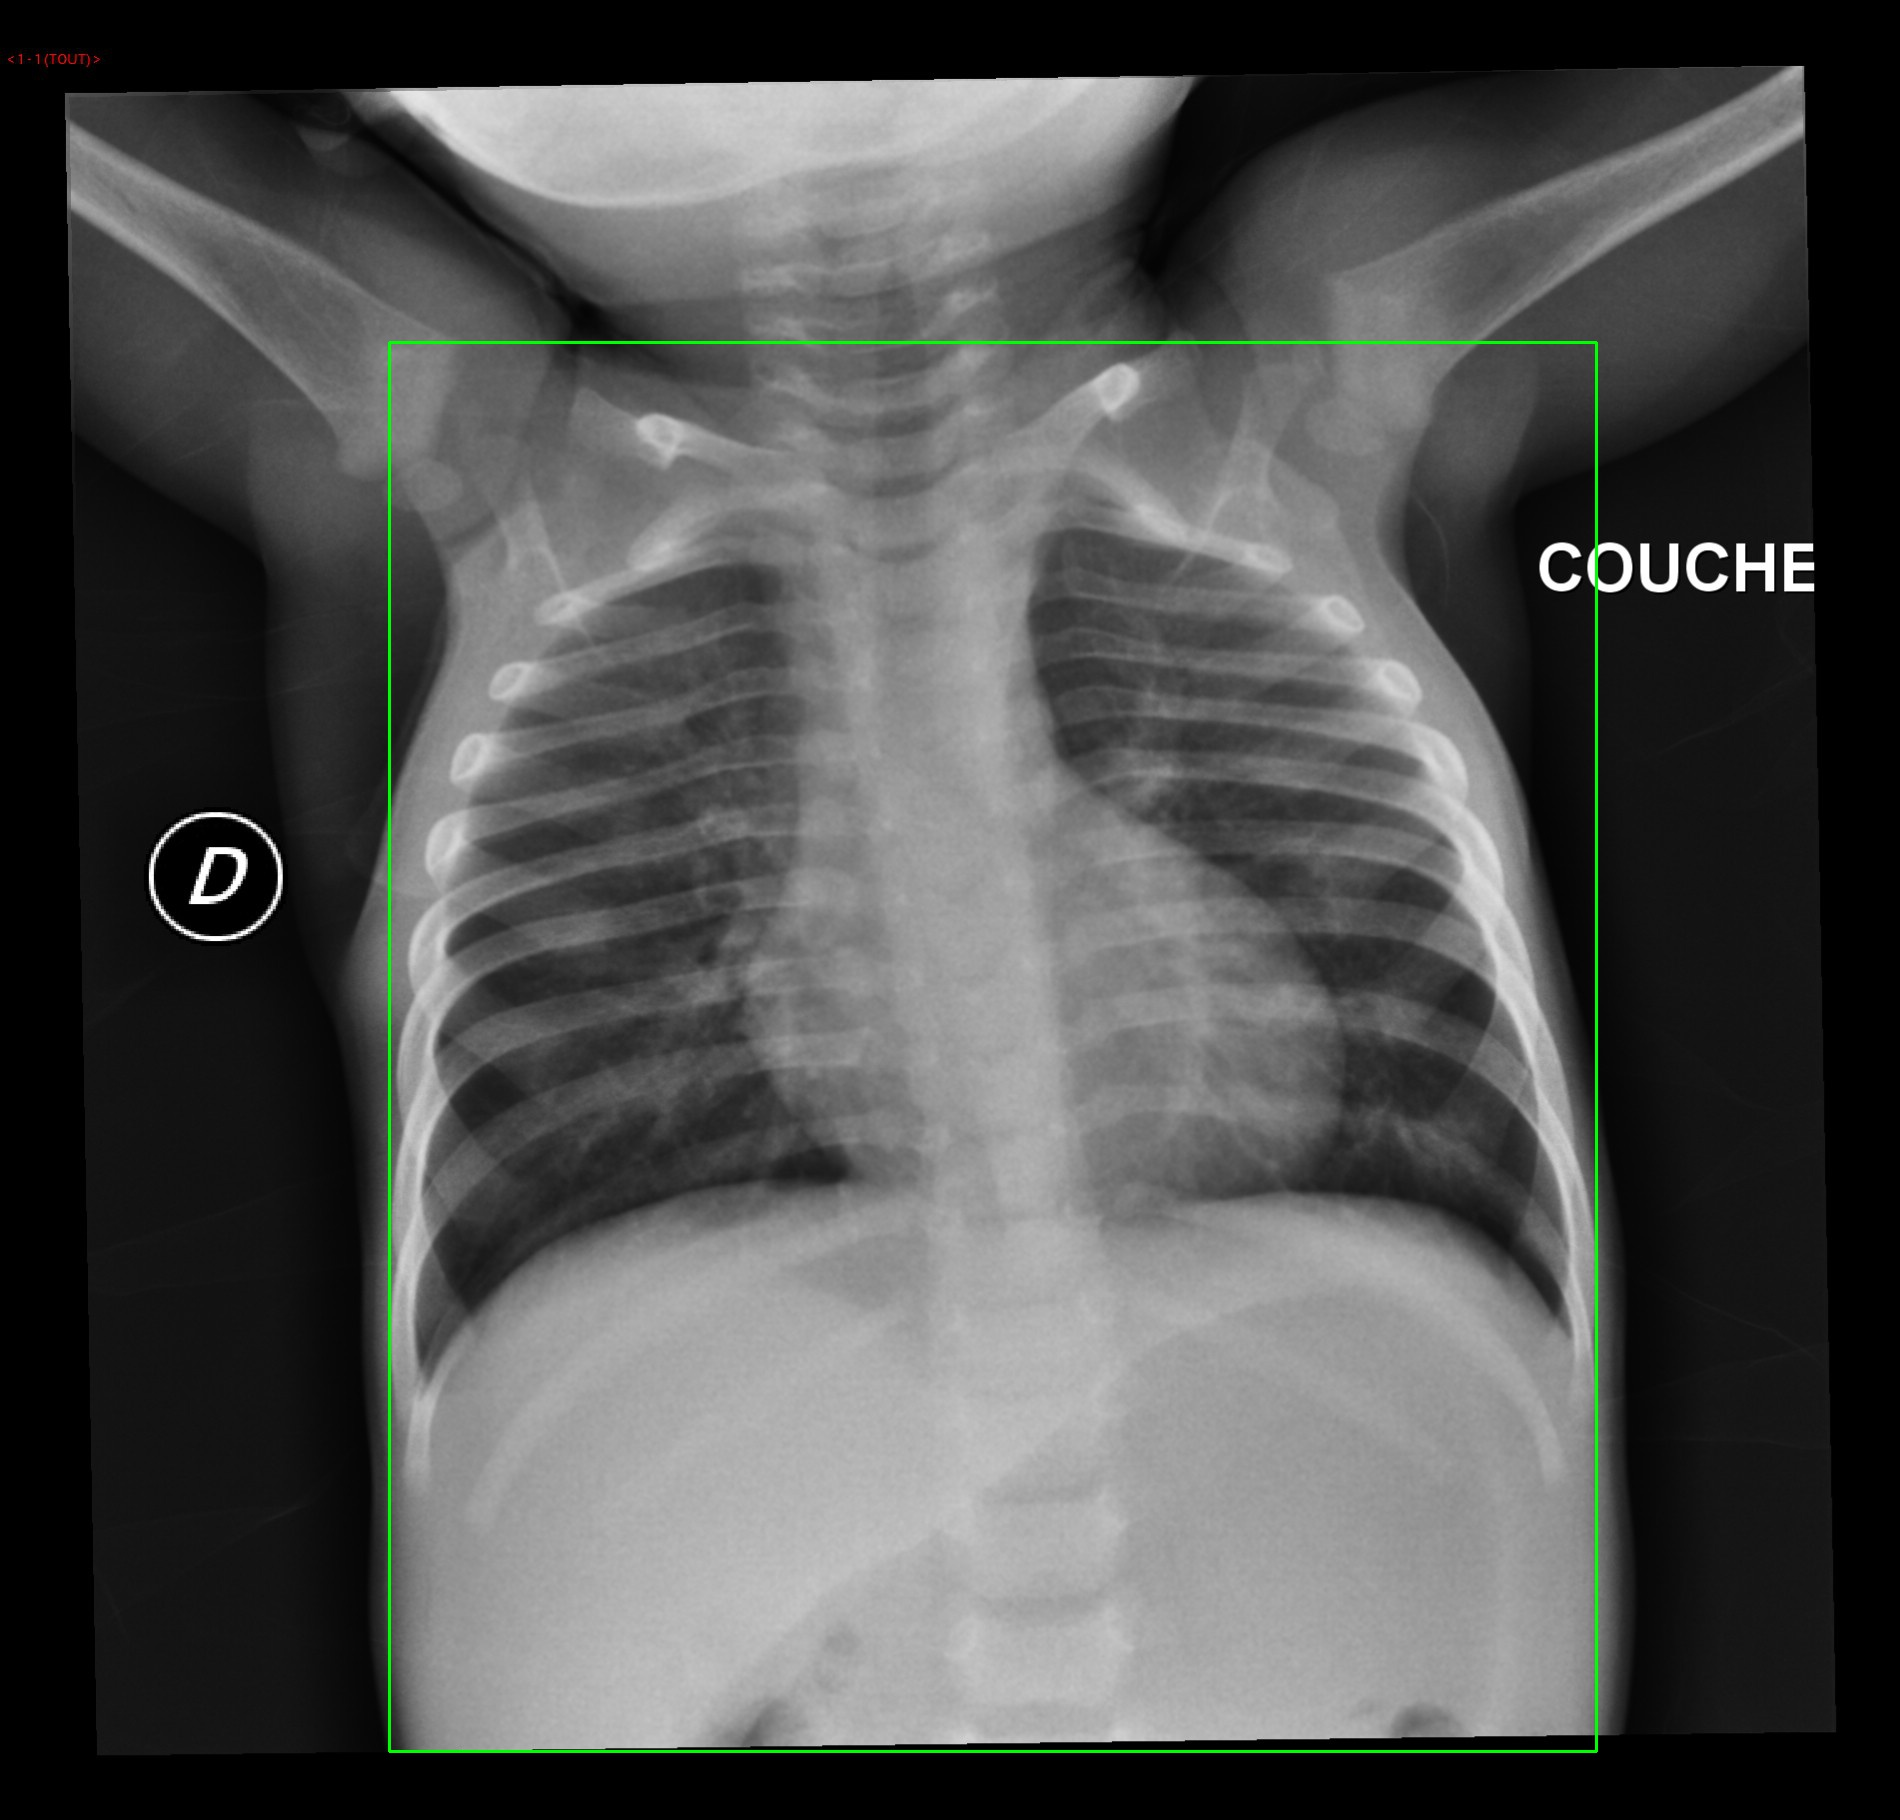
\includegraphics[scale=0.10]{boundingBoxRx1anNormale.jpg}
		\subcaption{RX normale}
	\end{minipage}
	\hfill
	\begin{minipage}[b]{.46\textwidth}
		\centering
		\includegraphics[scale=0.092]{boundingBoxRx4_5ansPneumopathieNecrosanteDroite.jpg}
		\subcaption{RX tuberculose}
	\end{minipage}
	\caption{Résultats: boîte englobant}
\end{figure}


Il reste d’autres  parties  du  corps  que les  poumons. La somme des valeurs des pixel sur chaque ligne a été calculé, ensuite la médiane de ces valeurs a été déterminé. Pour chaque ligne, si la valeur de  la  somme  sur  la  ligne  était  supérieure  à  la  médiane,  la  ligne  était  considérée  comme faisant  partie  du  poumon  sinon  elle  était  considérée  comme  faisant  partie  de  la  partie inférieure de l’image, majoritairement en noir sur les images considérées. Les résultats sont dans le Figure 2.3.

\begin{figure}[ht]
	\begin{minipage}[b]{.5\textwidth}
		\centering
		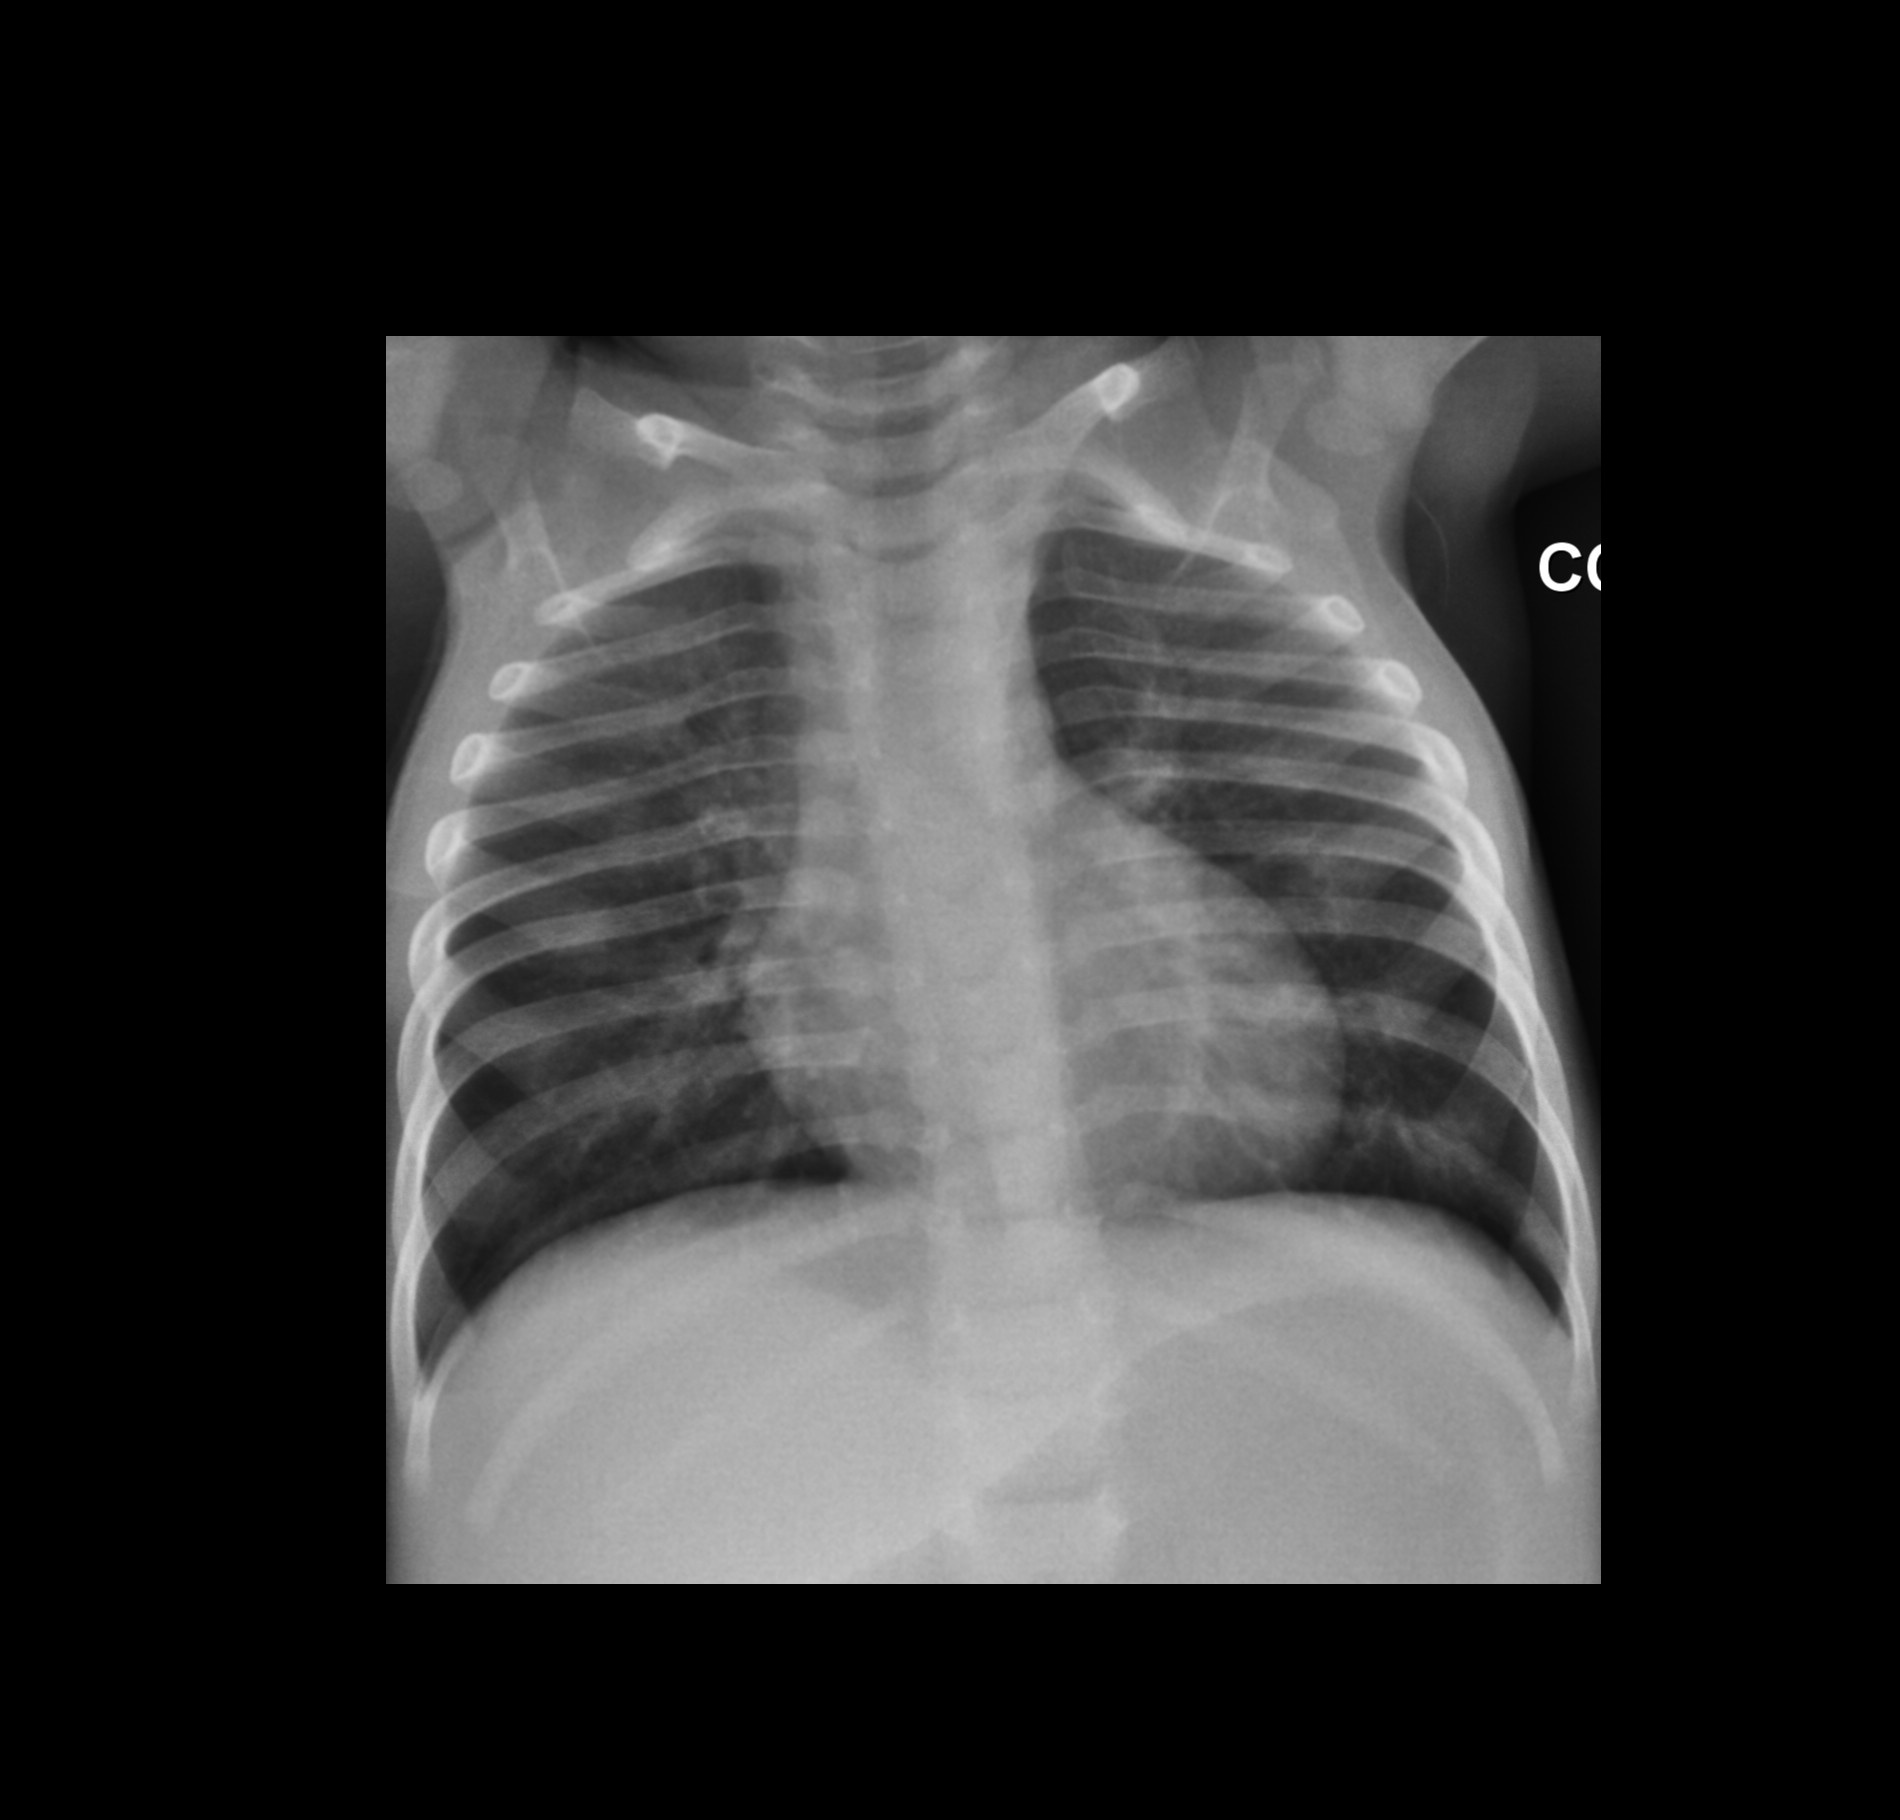
\includegraphics[scale=0.10]{lungsonly_Rx1anNormale.jpg}
		\subcaption{RX normale}
	\end{minipage}
	\hfill
	\begin{minipage}[b]{.46\textwidth}
		\centering
		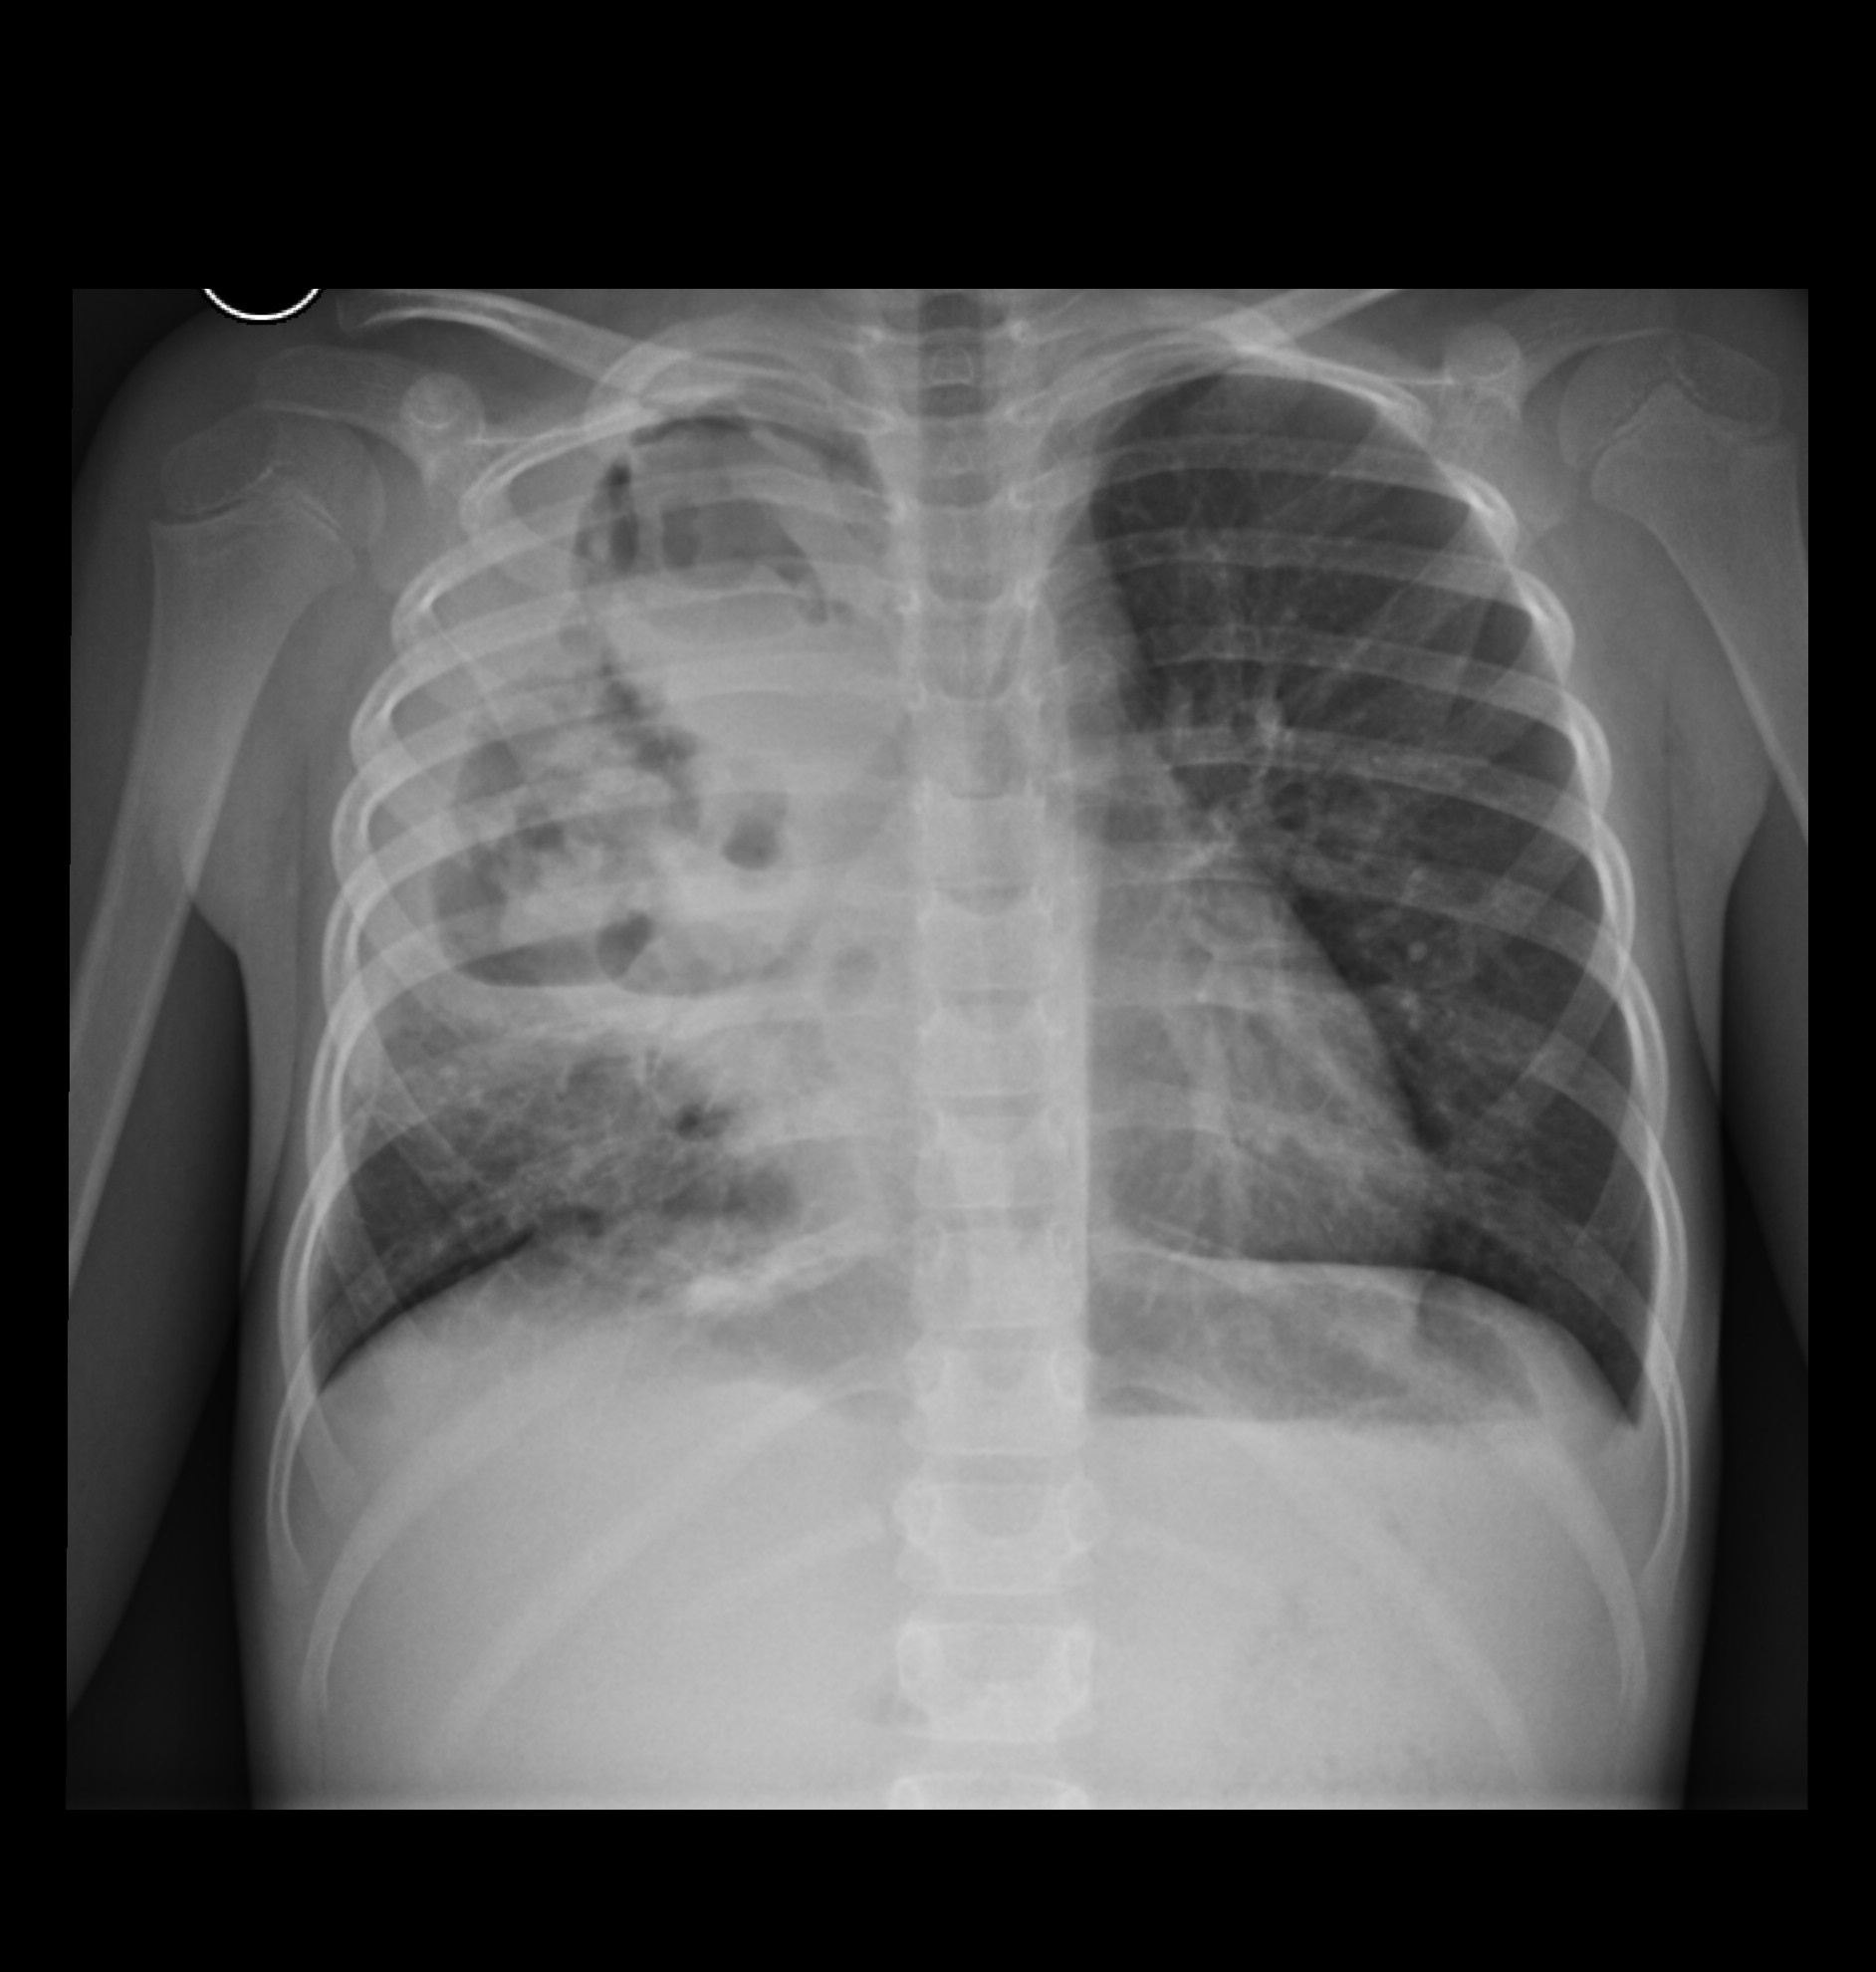
\includegraphics[scale=0.092]{lungsonly_Rx4_5ansPneumopathieNecrosanteDroite.jpg}
		\subcaption{RX tuberculose}
	\end{minipage}
	\caption{Résultats: lignes en noir}
\end{figure}
C'est possible apercevoir qu'il reste encore parties non désirs dans les RX. Un seuillage par hystérésis pour améliorer notre détection a été essayé aussi. Cependant, il y a eu des problèmes avec cette méthode, ce n'existait pas vraiment de modes distinguables dans l’histogramme.

 \pagebreak
 
\section{Identifier les anomalies}
Une idée très simple pour détecter les anomalies est comparer les deux poumons entre si. Pour faire cette comparaison  l'algorithme K-means a été utilisé. 
  Pour  chaque  image  la  valeur  associée  a été relevé à  chacune  des 
classes  (un  tableau  pour  la  classe  0,  un  tableau  pour  la  classe  1,  etc),  puis  la  valeur  moyenne a été calculé  des  valeurs  de  chaque classe.  Ensuite,  les valeurs ont été comparés  dans  la  classe,  dans  chaque  image,  à  cette  moyenne:  si  elle  lui  est  supérieure  on considère qu’il y a une anomalie. Il est possible de regarder ces résultats dans le Table 2.1.

\begin{table}[h]
	\centering

	\label{my-label}
	\begin{tabular}{llll|c|l|l|l|l|}
		\cline{5-9}
		&     &     &     & \multicolumn{5}{c|}{Base de données} \\ \hline
		\multicolumn{4}{|l|}{Faux positif} & \multicolumn{5}{c|}{2} \\ \hline
		\multicolumn{4}{|l|}{Faux négatif} & \multicolumn{5}{c|}{0} \\ \hline
		\multicolumn{4}{|l|}{Bon diagnostic} & \multicolumn{5}{c|}{75\%} \\ \hline
	\end{tabular}
	\caption{Résultats obtenus avec le méthode \textit{Kmeans}}
	\end{table}

Il est possible conclure que c'est premier analyse est très effectif, parce que tous les poumons avec tuberculose sont détectes, malgré les faux positif, parce que les faux positif peuvent être retirer dans analyses posteriori.

 HISTOGRAMME ?
\section{Détecter le tuberculose}
 Le premier difficulté trouvé était qu'il existe différents types de tuberculose et chaque une a ses propres caractéristiques et dans le même type de tuberculose il existe plusieurs identificateurs.
 
 REGARDER LES DIRECTIONS PRIVILEGIES
 
 ESSAYER DE COMPARER LES REGIONS QU'ON A APPERÇU DIF DANS LE HISTO
 
  TENSEURS?
\chapter {Conclusion}
\chapter*{Références bibliographiques}
\begin{enumerate}
	\item Satoshi Suzuki and others. Topological structural analysis of digitized binary images by border following. Computer Vision, Graphics, and Image Processing, 30(1):32–46, 1985.
	\item article isabelle bloch debut
	\item article isabelle bloch tenseurs
	
\end{enumerate}
 
\end{document}          
